\documentclass[utf8,english]{gradu3}
% If you are writing a Bachelor's Thesis, use the following instead:
%\documentclass[utf8,bachelor,english]{gradu3}

\usepackage{graphicx} % for including pictures

\usepackage{amsmath} % useful for math (optional)

\usepackage{booktabs} % good for beautiful tables

% NOTE: This must be the last \usepackage in the whole document!
\usepackage[bookmarksopen,bookmarksnumbered,linktocpage]{hyperref}

\graphicspath{ {img/} }
\addbibresource{bibliography.bib} % The file name of your bibliography database

\begin{document}

\title{Migrating a web application to serverless architecture}
\translatedtitle{Web-sovelluksen siirtäminen serverless-arkkitehtuuriin}
\studyline{Master's Thesis in Information Technology}
\avainsanat{%
  serverless,
  FaaS,
  arkkitehtuuri,
  pilvilaskenta,
  web-sovellukset}
\keywords{
  serverless,
  FaaS,
  architecture,
  cloud computing,
  web applications}
\tiivistelma{%
  Tämä kirjoitelma on esimerkki siitä, kuinka
  {gradu3}-tutkielmapohjaa käytetään.  Se sisältää myös
  käyttöohjeet ja tutkielman rakennetta koskevia ohjeita.

  Tutkielman tiivistelmä on tyypillisesti lyhyt esitys, jossa
  kerrotaan tutkielman taustoista, tavoitteesta, tutkimusmenetelmistä,
  saavutetuista tuloksista, tulosten tulkinnasta ja johtopäätöksistä.
  Tiivistelmän tulee olla niin lyhyt, että se, englanninkielinen
  abstrakti ja muut metatiedot mahtuvat kaikki samalle sivulle.

  Sen tulee kertoa täsmälleen samat asiat kuin englannikielinen
  abstrakti.
}
\abstract{%
  This document is a sample {gradu3} thesis document class
  document.  It also functions as a user manual and supplies
  guidelines for structuring a thesis document.

  The abstact is typically short and discusses the background, the
  aims, the research methods, the obtained results, the interpretation
  of the results and the conculsions of the thesis.  It should be so
  short that it, the Finnish translation, and all other meta
  information fit on the same page.

  The Finnish tiivistelmä of a thesis should usually say exactly the same
  things as the abstract.
}

\author{Aleksi Pekkala}
\contactinformation{\texttt{alvianpe@student.jyu.fi}}
% use a separate \author command for each author, if there is more than one
\supervisor{Oleksiy Khriyenko}
% use a separate \supervisor command for each supervisor, if there
% is more than one

\maketitle

% \begin{thetermlist}
% \item[FaaS] Function as a Service.
% % \item[\LaTeX] A system, built on top of \TeX\
% %   \parencite{knuth86:_texbook}, for typesetting structured
% %   documents \parencite[see][]{lamport94:_latex}.  Its current version
% %   is \LaTeXe.
% \end{thetermlist}

\mainmatter

\chapter{Introduction}

Cloud computing has in the past decade emerged as a veritable backbone of modern economy, driving innovation both in industry and academia as well as enabling scalable global enterprise applications. Just as the adoption of cloud computing continues to increase, the technologies in which the paradigm is based have continued to progress. Recently the development of novel virtualization techniques has lead to the introduction of \textit{serverless computing}, an architectural pattern based on ephemeral cloud resources that scale up and down automatically and are billed for actual usage at a millisecond granularity. The main drivers behind serverless computing are to both reduce operational costs by more efficient cloud resource utilization and to improve developer productivity by shifting provisioning, load balancing and other infrastructure concerns to the platform. \parencite{buyya2017manifesto}

As an appealing economic proposition, serverless computing has attracted significant interest in the industry. This is illustrated for example by its appearance in the 2017 Gartner Hype Technologies Report \parencite{walker17gartnerHype}. By now most of the prominent cloud service providers have introduced their own serverless platforms, promising capabilities that make writing scalable web services easier and cheaper \parencite[e.g.][]{awslambda0218, google18cloudFunctions, ibm18cloudFunctions, microsoft18azureFunctions}. A number of high-profile use cases have also been presented in the literature \parencite{cncf18serverlessWG}. \textcite{baldini17currentTrends} however note a lack of corresponding degree of interest in academia despite a wide variety of technologically challenging and intellectually deep problems in the space.

One of the open problems identified in literature concerns the discovery of serverless design patterns: how do we compose the granular building blocks of serverless into larger systems? \parencite{baldini17currentTrends} \textcite{varghese18next} contend that one challenge hindering the widespread adoption of serverless will be the radical shift in the properties that a programmer will need to focus on, from latency, scalability and elasticity to those relating to the modularity of an application. Considering this and the paradigm's unique characteristics and limitations, it's unclear to what extent our current patterns apply and what kind of new patterns are best suited to optimize for the features of serverless computing. The object of this thesis is to fill the gap by re-evaluating existing design patterns in the serverless context and proposing new ones through an exploratory migration process.

\section{Research problem}

The research problem addressed by this thesis distills down to 4 different questions:
\begin{enumerate}
  \item Why should a web application be migrated to serverless?
  \item What kind of patterns are there for building serverless web application backends?
  \item Do the existing patterns have gaps or missing parts, and if so, can we come up with improvements or alternative solutions?
  \item How does migrating a web application to serverless affect its quality?
\end{enumerate}

The first two questions are addressed in the theoretical part of the thesis. Question 1 concerns the motivation behind the thesis and introduces serverless migration as an important and relevant business problem. Question 2 is answered by surveying existing literature for serverless patterns as well as other, more general patterns thought suitable for the target class of applications.

The latter questions form the constructive part of the thesis. Question 3 concerns the application and evaluation of surveyed patterns. The surveyed design patterns are used to implement a subset of an existing traditional web application in the serverless architecture. In case the patterns prove unsuitable for any given problem, alternative solutions or extensions are proposed. The last question consists of comparing the migrated portions of the app to the original version and evaluating whether the posited benefits of serverless architecture are in fact realized.

\section{Outline}

The thesis is structured as follows: the second chapter serves as an introduction to the concept of serverless computing. The chapter describes the main benefits and drawbacks of the platform, as well as touching upon its internal mechanisms and briefly comparing the main service providers. Extra emphasis is placed on how the platform's limitations should be taken into account when designing web application backends.

The third chapter consists of a survey into existing serverless design patterns and recommendations. Applicability of other cloud computing, distributed computing and enterprise integration patterns is also evaluated.

The fourth chapter describes the process of migrating an existing web application to serverless architecture. The patterns discovered in the previous chapter are utilized to implemented various typical web application features on a serverless platform. In cases where existing patterns prove insufficient or unsuitable as per the target application's characteristics, modifications or new patterns are proposed.

The outcome of the migration process is evaluated in the fifth chapter. The potential benefits and drawbacks of the serverless platform outlined in chapter 2 are used to reflect on the final artifact. The chapter includes approximations on measurable attributes such as hosting costs and performance as well as discussion on the more subjective attributes like maintainability and testability. The overall ease of development -- or developer experience -- is also addressed since it is one of the commonly reported pain points of serverless computing \parencite{van2017spec}.

The final chapter of the thesis aims to draw conclusions on the migration process and the resulting artifacts. The chapter contains a summary of the research outcomes and ends with recommendations for further research topics.


\chapter{Serverless computing}

This chapter serves as an introduction to serverless computing. We approach the formidable task of defining serverless by distinguishing between its two main approaches. After that we'll go over the background and motivations behind the serverless paradigm. This is followed by a look at the basic features of a serverless runtime, as well as the major providers and use cases. The chapter closes with notes on the drawbacks and limitations of serverless, particularly from the point of view of web application backends.

Defining serverless computing succinctly can be difficult because of the relative immaturity of the field and the fact that there's significant overlap with other cloud computing terms. To complicate matters further, serverless computing has come to appear in two different but overlapping forms. The term 'serverless' in itself can also seem a bit disingenuous, since despite the name serverless computing obviously still involves servers. The name -- coined by industry -- instead implies that there's no longer need for the developer to spend time and resources on managing servers.

\section{Defining serverless}

% Defining serverless computing succinctly can be difficult because of the relative immaturity of the field and the fact that there's significant overlap with other cloud computing terms. To complicate matters further, serverless computing has come to appear in two different but overlapping forms: Backend-as-a-Service (BaaS) as well as Function-as-a-Service (FaaS) \parencite{buyya2017manifesto}. Fundamentally serverless computing is about building and running back-end code that does not require server management or server applications \parencite{robert2016serverlessarchitectures}. The two forms of serverless computing, as described in section \ref{baasVSfaas}, serve this same purpose with two different approaches.

% The term 'serverless' in itself can also seem a bit disingenuous, since despite the name serverless computing obviously still involves servers. The name -- coined by industry -- instead implies that there's no longer need to spend time and resources on managing servers. Tasks such as provisioning, maintenance and capacity planning are handled by the serverless platform as needed by current workload. This leaves developers to focus on application logic, providing an abstraction where computation is disconnected from the infrastructure it is going to run on. \textcite{van2017spec} further define serverless computing by three key characteristics:

Fundamentally serverless computing is about building and running back-end code that does not require server management or server applications \parencite{robert2016serverlessarchitectures}. The two forms of serverless computing, as described in section \ref{baasVSfaas}, serve this same purpose with two different approaches. The two serverless models, while different in operation, are nonetheless grouped under the same serverless umbrella since they both deliver the same main benefits: zero server maintenance overhead and the elimination of idle costs \parencite{cncf18serverlessWG}.

\begin{enumerate}
  \item Granular billing: the user of a serverless model is charged only when the application is actually executing
  \item (Almost) no operational logic: operational logic, such as resource management and autoscaling, is delegated to the infrastructure, making those concerns of the infrastructure operator
  \item Event-driven: interactions with serverless applications are designed to be short-lived, allowing the infrastructure to deploy serverless applications to respond to events, so only when needed
\end{enumerate}


%As a sidenote, although the earliest uses of term 'serverless' can be traced back to peer-to-peer and client-only solutions \parencite{fox17}, we're dismissing these references since the name has evolved into a completely different meaning in the current cloud computing context.


TODO: How does serverless relate to concepts such as FaaS, BaaS/MBaaS like Auth0 and Firebase, SOA, microservices, event-driven, virtualization, containers, cloud-native, ...? Cloud-ready/cloud-native as defined by \textcite{pozdniakova17cloudready}.

% \textcite{fox17} present a useful short definition of serverless as a cloud-native platform for short-running, stateless computation and event-driven applications which scales up and down instantly and automatically and charges for actual usage at a millisecond granularity.

\section{BaaS and FaaS} \label{baasVSfaas}

Backend-as-a-Service refers to an architecture where an application's server-side logic is replaced with external cloud services that carry out various tasks like authentication or database access \parencite{buyya2017manifesto}. The model -- also known as Mobile-Backend-as-a-Service (MBaaS) \parencite{sareen13cloudTypes} -- is typically utilized in the mobile space to avoid having to manually set up and maintain server resources for the more narrow back-end requirements of a mobile application. The application's core business logic is implemented client-side and integrated tightly with third party remote application services. Since these API-based BaaS services are managed transparently by the cloud service provider, the model appears to the developer to be serverless.

Function-as-a-Service is a more recent development: the first commercial FaaS platform, AWS Lambda, was introduced in November 2014 \parencite{awslambda0218}. In the FaaS architecture an application's business logic is still located server-side. The crucial difference is that instead of self-managed server resources, developers upload small units of code to a FaaS platform that executes the code in short-lived, stateless compute containers in response to events \parencite{robert2016serverlessarchitectures}. The model appears serverless in the sense that the developer has no control over the resources on which the back-end code runs. \textcite{albuquerque17faaspaas} note that the BaaS model of locating business logic on the client side carries with it some complications, namely difficulties in updating and deploying new features as well as reverse engineering risks. FaaS circumvents these problems by retaining business logic server-side.

Another perspective on the difference between the two serverless models is to view BaaS as a more tailored, vendor-specific approach to FaaS \parencite{van2017spec}. Whereas BaaS-type services function as built-in components for many common use cases such as user management and data storage, a FaaS platform allows developers to implement more customized functionality. This thesis focuses on the latter, since out of the two models FaaS is the one with significant differences to traditional web application architecture (as illustrated later) and thus more interesting concerning the research questions in hand. BaaS however plays an important role in serverless architectures as it will often be the supporting infrastructure (e.g. in form of data storage) to the stateles FaaS functions \parencite{cncf18serverlessWG}. Conversely, in case of otherwise BaaS-based applications there's likely still a need for custom server-side functionality; FaaS functions may be a good solution for this \parencite{robert2016serverlessarchitectures}. Serverless applications can utilize both models simultaneously, with BaaS platforms generating events that trigger FaaS functions, and FaaS functions can acting as a 'glue component' between various third party BaaS services.  \textcite{robert2016serverlessarchitectures} also notes convergence in the space, giving the example of the user managemement provider Auth0 starting initially with a BaaS-style offering but later entering the FaaS space with a 'Auth0 Webtask' service.

Add sidenote about the apparent confusion with these terms: at least \textcite{baldini17currentTrends} and \textcite{varghese18next} seem to consider 'serverless' to equal FaaS, excluding BaaS.

\section{Comparison to other cloud computing models}

\begin{quote}
As serverless is gaining popularity the boundaries between different types of ”as-a-Service” may be disappearing (see Figure 9). One could imagine that developersnot only write code but also declare how they want the code to run - as FaaS orMBaaS or PaaS - and can change as needs change. In the future the main distinc-tion may be between caring about server (server-aware) and not caring about serverdetails (server-less). PaaS is in the middle; it makes it very easy to deploy code butdevelopers still need to know about servers and be aware of scaling strategies, suchas how many instances to run. \parencite{baldini17currentTrends}
\end{quote}

\textcite{van2017spec} in turn note that some PaaS/SaaS offerings such as Auth0 and FaunaDB, although not generally considered serverless, exhibit the main characteristics of serverless.

\begin{figure}[h]
  \centering
  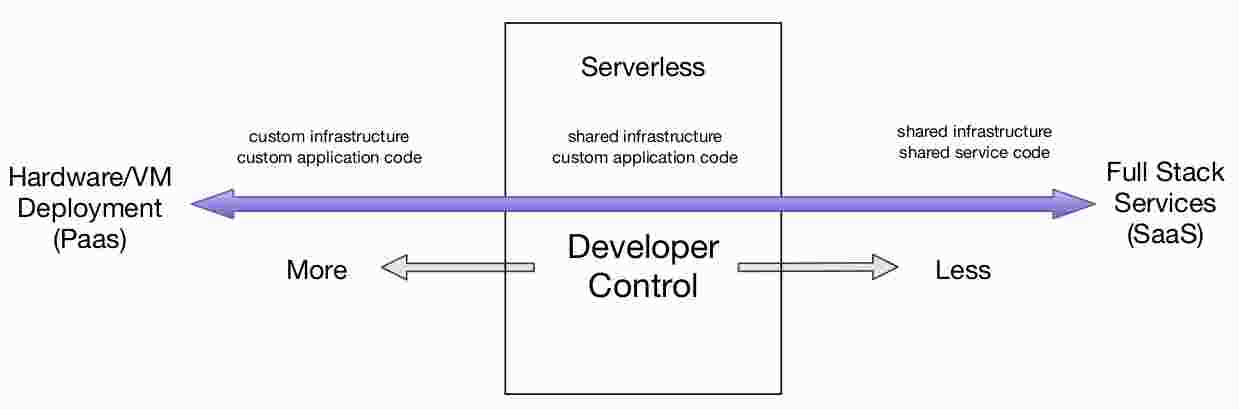
\includegraphics[width=\textwidth]{baldini17-paas-faas-saas.jpg}
  \caption{Developer control and serverless computing \parencite{baldini17currentTrends}}
\end{figure}

\section{Serverless application architecture}

\textcite{van2017spec} on serverless and SOA architecture: We see the emerging model based on running individual cloud functions as a consequence of the slow but sustained evolution of computing. For many decades we have witnessed a transition from relatively large, monolithic applications, to smaller or more struc- tured applications with smaller execution units (e.g, workflows with many small tasks). This transition is captured qualitatively by vari- ous software architectures, for example, the Service-Oriented Ar- chitecture, and quantitatively by various workload-characterization and modeling studies, for example of scientific workloads running on supercomputers and grids between 1990 and 2010.

% Historical/evolutionary views: 1) on-premises infra -> grid -> IaaS -> PaaS -> serverless, 2) bare metal -> VMs -> containers -> functions \parencite{fox17}, 3) monolith -> SOA -> microservices -> serverless.

\section{Background}

The vision of computing as an utility can be dated back to at least 1969 and ARPANET. \parencite{buyya09cloud}

Cloud computing is by now a well-established paradigm that enables organizations to flexibly deploy their software systems over a pool of computing resources.  \parencite{jamshidi13cloudmigrationreview}

The motivations behind cloud migration in general. \textcite{jamshidi13cloudmigrationreview} identify cost saving, scalability, and efficient utilization of resources as well as flexibility as key drivers to migrate application to the cloud. \textcite{balalaie16migratingcloud} talk about the reasons behind migrating systems to cloud-native architectures.

\textcite{youseff08cloudOntology} with a detailed ontology of cloud computing. The recent evolution of cloud computing has borrowed its basics from several other computing areas and systems engineering concepts. Cluster and Grid Computing on one hand, and virtualization on the other hand are perhaps the most obvious predecessor technologies that enabled the inception of cloud computing. However, several other computing concepts have indirectly shaped today's cloud computing technology, including peer-to-peer (P2P) computing, SOA and autonomic computing.

Serverless platforms promise new capabilities that make writing scalable mi-
croservices easier and cost effective, positioning themselves as the next step in the
evolution of cloud computing architectures. \parencite{baldini17currentTrends}

reason behind cloud migration, why is cloud important? organizations migrate to cloud because of A, B, C... note reasons why NOT to migrate to cloud and whether they also apply to serverless.

Another particularly important reason is... Particular importance in the current energy-constrained environment. Data centers use on the order of 1-2\% of global energy consumption, but server utilization rates are really low. \parencite{horner16powerusage}

historically cloud has been driven by virtualization, IaaS to PaaS to CaaS...

serverless takes these benefits to the extreme... how does serverless work and lean on the existing technology, compare to other platforms

\section{Use cases}

Introduce the main/intended use cases for serverless, as well as the more esoteric applications in literature.

\textcite{malawski17executescientific} find that while serverless infrastructures are designed mainly for processing background tasks of Web and IoT applications, the simple mode of operation makes this approach easy to use and promising in scientific workflows too. \textcite{jonas17occupy} argue that a serverless execution model with stateless functions can enable radically-simpler, fundamentally elastic, and more user-friendly distributed data processing systems. \textcite{spillner18faaster} also find that in many domains of scientific and high-performance computing, solutions can be engineered based on simple functions which are executed on commercially offered or self-hosted FaaS platforms.

Introduce edge computing as a particularly strong driver for serverless. \textcite{glikson17devicelessedge} propose the novel paradigm of Deviceless Edge Computing that extends the serverless paradigm to the edge of the network, enabling IoT and Edge devices to be seamlessly integrated as application execution infrastructure. \textcite{nastic17analyticsedge} present a novel approach implementing cloud-supported, real-time data analytics in serverless edge-computing applications. \textcite{baresi17edgecomputing} propose a serverless architecture at the edge, bringing a highly scalable, intelligent and cost-effective use of edge infrastructure’s resources with minimal configuration and operation efforts.

\textcite{fouladi2017encoding} present a serverless video-processing framework. \textcite{yan16chatbot} present the architecture and prototype of a chatbot using a serverless platform, where developers compose stateless functions together to perform useful actions. \textcite{ishakian17neural} evaluate the suitability of a serverless computing environment for the inferencing of large neural network models. \textcite{ast17webcomponent} describe an approach of how to utilize serverless computing to enable self-contained web components by deploying Web Component business logic as cloud-hosted functions.

\section{Runtime}

Briefly describe the inner workings of a FaaS runtime. Describe the two supported execution models, synchronous and asynchronous, and how they relate to application design. The former is used to build a typical request-response flow, e.g. a REST API endpoint, whereas the latter relates to pub-sub and other event-driven flows. Give examples on the kind of triggers supported by serverless platforms (HTTP calls, messaging, database events, ...).

\textcite{spillner17snafu} presents the design and implementation of a research-friendly FaaS runtime. \textcite{mcgrath17implement} present the design of a novel performance-oriented serverless computing platform, discussing implementation challenges such as function scaling and container discovery, lifecycle, and reuse. \textcite{hendrickson16openlambda} present OpenLambda, an open-source platform for serverless computation, describing the key aspects of serverless computation and presenting numerous research challenges that must be addressed in the design and implementation of such systems.

\section{Service providers}

\textcite{lynn2017preliminary} provide an overview and multi-level feature analysis of seven enterprise serverless computing platforms. \textcite{baldini17currentTrends} also has a narrower survey of serverless platforms.

\section{Economics of serverless}

\textcite{eivy2017wary} and \textcite{villamizar2016infrastructure} both focus on the economic aspects of serverless. \textcite{adzic2017serverless} explain how novel design patterns are used to significantly optimize costs -- just running traditional web apps inside Lambda containers doesn't necessarily equate to savings. \textcite{adzic2017serverless} also report savings between 66 and 95\% in two case studies, and present a handly table comparing hosting prices for intermittent service tasks. \textcite{spillner17exploiting} exploits the control plane of AWS Lambda to implement services practically for free. \textcite{leitner16modelcost} present an approach to model deployment costs of AWS Lambda applications in real-time. \textcite{kuhlenkamp17costradamus} present another cost-tracing system that enables per-request cost-tracing for cloud-based software services, noting that cost testing should not only rely on isolated tests of single services but consider comprehensive end-to-end cost traces. \textcite{albuquerque17faaspaas} have a detailed price comparison running the same app in FaaS and PaaS.

\section{Security}

Address the security implications of serverless. Overall the consensus seems to be that compared to services maintaining their own servers and resources, serverless approach reduces the attack surface However, research needs to understand the new security issues introduced by FaaS. For example, because the infrastructure can share resources among cloud-functions, what is the ideal security vs. performance/cost trade-off? \parencite{van2017spec}

\section{Drawbacks and limitations}

What to take into consideration when migrating to serverless?

\textcite{lloydserverless} analyze serverless performance and elasticity, identifying the cold start phenomenon. Differences in runtimes/languages, and larger library dependencies lead to slower starts. \textcite{oakes17pipsqueak} address the problem by caching package dependencies on platform-level.

\textcite{baldini17trilemma} identify three competing constraints in serverless function composition: functions should be considered as black boxes; function composition should obey a substitution principle with respect to synchronous invocation; and invocations should not be double-billed.

\textcite{robert2016serverlessarchitectures}, \textcite{adzic2017serverless} and \textcite{baldini17currentTrends} each list a number of limitations, including lack of strong SLA, vendor lock-in, short life-span, immature local development tools, statelessness and many others.

\textcite{kuhlenkamp17costradamus} discover two serverless cost tradeoffs: the retry cost effect and the cost ripple effect.

The need for circuit breakers (risk of DDoSing yourself) when interacting with non-serverless components like a database. Mention novel cloud-native database services like Google's Cloud Spanner and AWS Aurora. Figure out a source for this -- \textcite{hohpe2004enterprise} might have a relevant pattern.

Address maintainability: debugging serverless functions, following the flow of control can be tough.

Composing serverless functions is not like composing regular functions. All the difficulties of distributed computing -- message loss, timeouts and others -- apply and have to be handled. Possible solutions include retry policies, dead-letter queues and idempotent functions.

\chapter{Serverless design patterns}

Survey of serverless design patterns. \textcite{baldini17currentTrends} put the question as follows:

\begin{quote}
Will there be patterns for building serverless solutions? How do we combine low granularity basic building blocks of serverless into bigger solutions? How are we going to decompose apps into functions so that they optimize resource usage? For example how do we identify CPU-bound parts of applications built to run in serverless services? Can we use well-defined patterns for composing functions and external APIs? What should be done on the server vs. client (e.g., are thicker clients more appropriate here)? Are there lessons learned that can be applied from OOP design patterns, Enterprise Integration Patterns, etc.?
\end{quote}

\section{Serverless patterns}

A limited number of purely serverless design patters. \textcite{sbarski2017serverless} introduce five patterns -- Command, Messaging Priority queue, Fan-out and Pipes and filters -- but they seem mostly to be reinterpretations of classic Enterprise Integration Patterns.

Common low-level design patterns such as function chaining and fanout \href{https://github.com/yochay/serverlesspatterns}{in Github}.

API Gateway and messaging patterns as described in platforms' own documentation. \parencite{awslambda0218}

\textcite{adzic2017serverless} suggest 3 methods for optimizing resource usage: use distributed authorization, let clients orchestrate workflows and allow clients to directly connect to AWS resources. The authors also discuss how paying only for actual utilization has two additional benefits of 1) removing incentives for bundling and 2) removing barriers to versioning: examples of serverless economics affecting architecture. Presenting these (or applications of these) as more formal patterns could be of some value.

\textcite{robert2016serverlessarchitectures} asks how big can FaaS functions get before they get unwieldy? Assuming we can atomically deploy a group of FaaS functions what are good ways of creating such groupings - do they map closely to how we’d currently clump logic into microservices or does the difference in architecture push us in a different direction? Extending this further what are good ways of creating hybrid architectures between FaaS and traditional ‘always on’ persistent server components?

Extending this further what are good ways of creating hybrid architect

\textcite{ast17webcomponent} describe self-contained web components with serverless backends.

\section{Enterprise Integration Patterns}

\textcite{hohpe2004enterprise} present a number of asynchronous messaging architectures in the seminal book on EIP. While predating the whole serverless phenomenon the patterns are still relevant. Hohpe even demonstrated implementing one of his patterns on top of Google's serverless platform \href{http://www.enterpriseintegrationpatterns.com/ramblings/google_cloud_functions.html}{in a blog post}.

\section{FaaSification}

\textcite{spillner17transformpython} describes an automated approach to transform monolithic Python code into modular FaaS units by partially automated decomposition. Doesn't really seem suitable for the web application migration process covered in this thesis but worth mentioning.

\chapter{Migration process}

Implement a subset of the target app in a serverless style, utilizing the surveyed patterns and keeping log of the tricky parts. In case the patterns prove unsuitable for the given problem, try to come up with an alternative solution.

Describe the web application to migrate.

Decide on the parts to migrate. Should demonstrate the features and limitations of serverless as outlined above. Possible features include
\begin{itemize}
  \item A simple REST API endpoint to showcase API Gateway and synchronous invocation. Shouldn't require any big changes to application code.
  \item Interaction between multiple services to demonstrate distributed transactions.
  \item A scheduled (cron) event.
  \item Interacting with an external SaaS service like Twilio, Auth0. Demonstrate event-driven invocation.
  \item others?
\end{itemize}

\chapter{Evaluation}

Evaluation the outcome of migration process. Estimate the effects on performance and hosting costs. Weigh in on maintainability, testability, developer experience etc.

\chapter{Conclusion}

What can we conclude about the research questions? Mention limitations and further research directions.

\printbibliography

\end{document}
